\chapter{Appendix 1} \label{app:whitening}

\begin{table} [h!]
    \begin{tabular}{ccc}
    Index & Abbreviation & Full form \\
    \hline
    0 & w/n & Whitening / No whitening \\
    1 & n/s/w/a & No filter / Static filter / Wiener filter / Adaptive filter \\
    2 & m/i/r & Moving average envelope / IIR LP envelope / RMS envelope \\
    \end{tabular}
    \caption{Table for clarifying the abbreviations used in result bar charts}
    \label{tab:abbreviation_explanation}
\end{table}

\begin{figure}[h!t]
	\begin{center}
		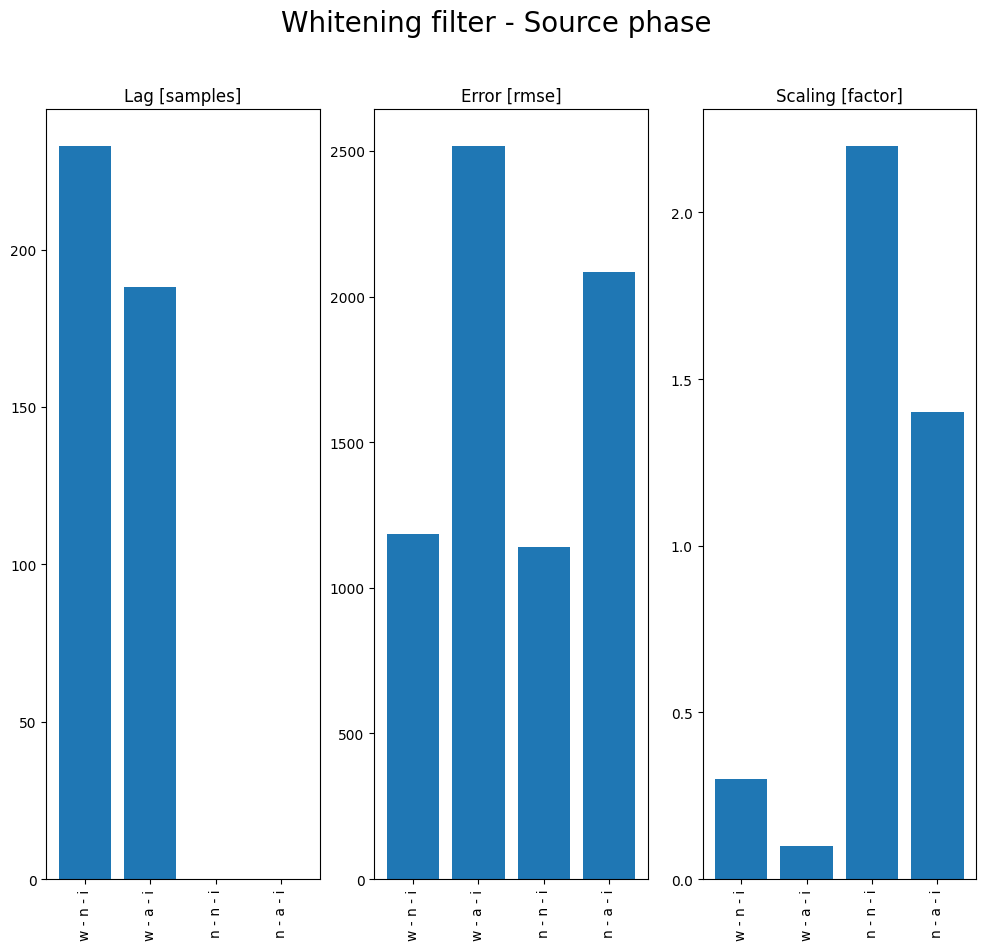
\includegraphics[width=1.0\columnwidth]{images/result_whitening_sourcephase.png}
	\end{center}
	\caption{Lag, error, and scaling of different filtering and envelope techniques with whitening applied. The whitening filter is constructed from the desired frequency amplitude response and a phase. The frequency response is determined as described in the simulation section \ref{sec:whitening}, and the phase is set to the phase of the input signal that was used to construct the whitening filter. The abbreviations are the first letter of the used technique for each step. Further clarification of these abbreviations can be found in Table~\ref{tab:abbreviation_explanation}}
	\label{fig:result_whitening_sourcephase}
\end{figure}

\begin{figure}[h!t]
	\begin{center}
		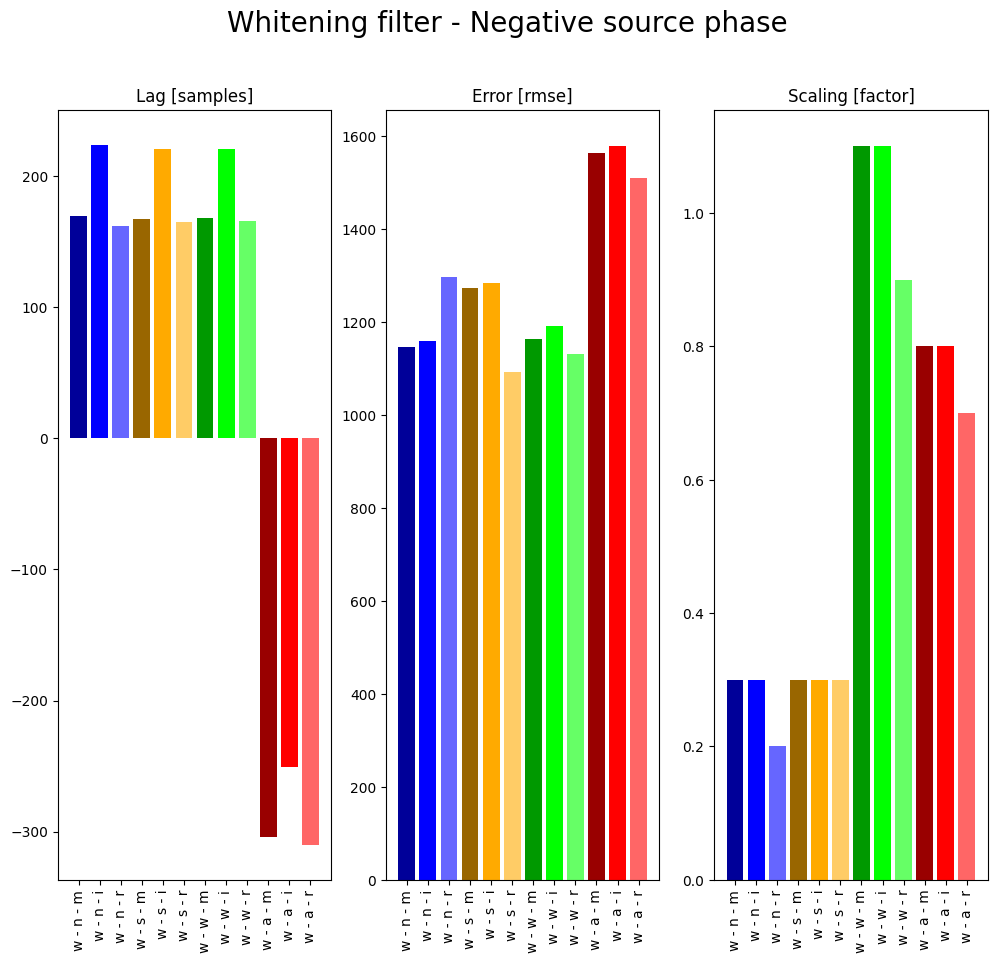
\includegraphics[width=1.0\columnwidth]{images/result_whitening_negative_sourcephase.png}
	\end{center}
	\caption{Lag, error, and scaling of different filtering and envelope techniques with whitening applied. The whitening filter is constructed from the desired frequency amplitude response and a phase. The frequency response is determined as described in the simulation section \ref{sec:whitening}, and the phase is set to the negative phase of the input signal that was used to construct the whitening filter. The abbreviations are the first letter of the used technique for each step. Further clarification of these abbreviations can be found in Table~\ref{tab:abbreviation_explanation}}
	\label{fig:result_whitening_negative_sourcephase}
\end{figure}

\begin{figure}[h!t]
	\begin{center}
		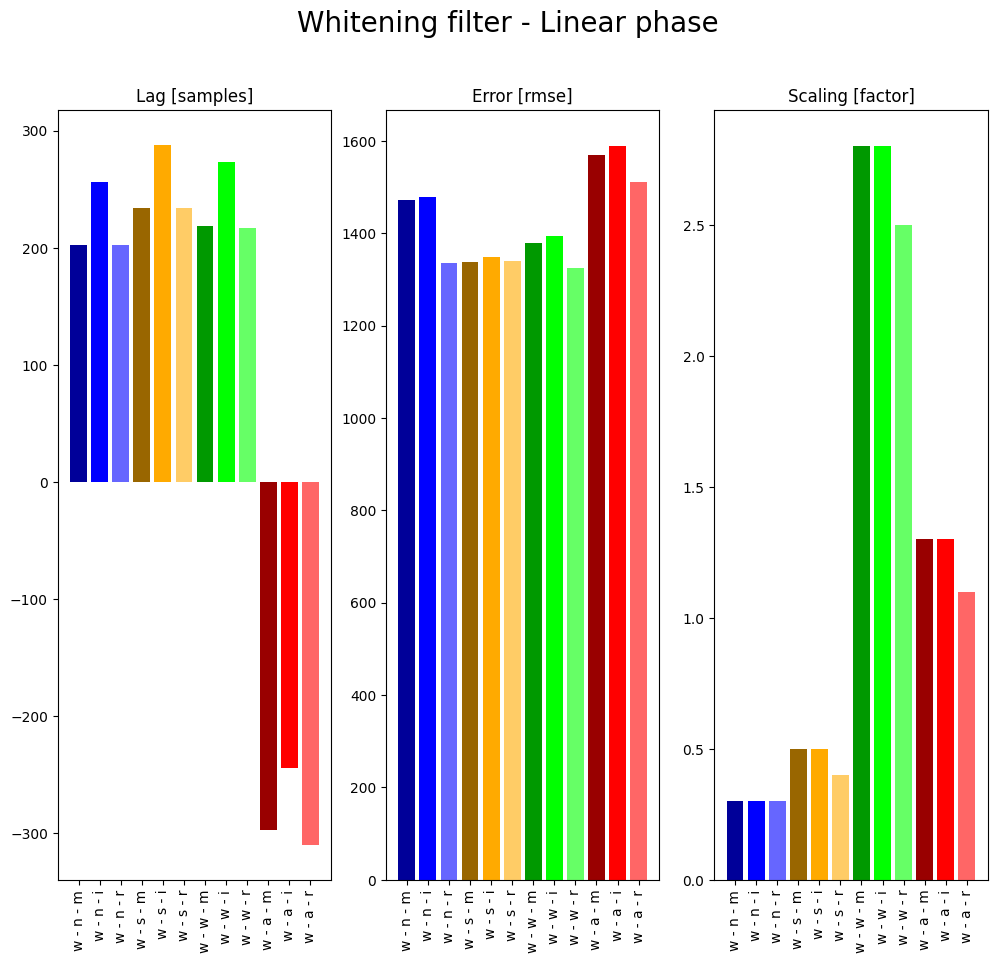
\includegraphics[width=1.0\columnwidth]{images/result_whitening_linearphase.png}
	\end{center}
	\caption{Lag, error, and scaling of different filtering and envelope techniques with whitening applied. The whitening filter is constructed from the desired frequency amplitude response and a phase. The frequency response is determined as described in the simulation section \ref{sec:whitening}, and the phase is set to linear phase. The abbreviations are the first letter of the used technique for each step. Further clarification of these abbreviations can be found in Table~\ref{tab:abbreviation_explanation}}
	\label{fig:result_whitening_linearphase}
\end{figure}

\begin{figure}[h!t]
	\begin{center}
		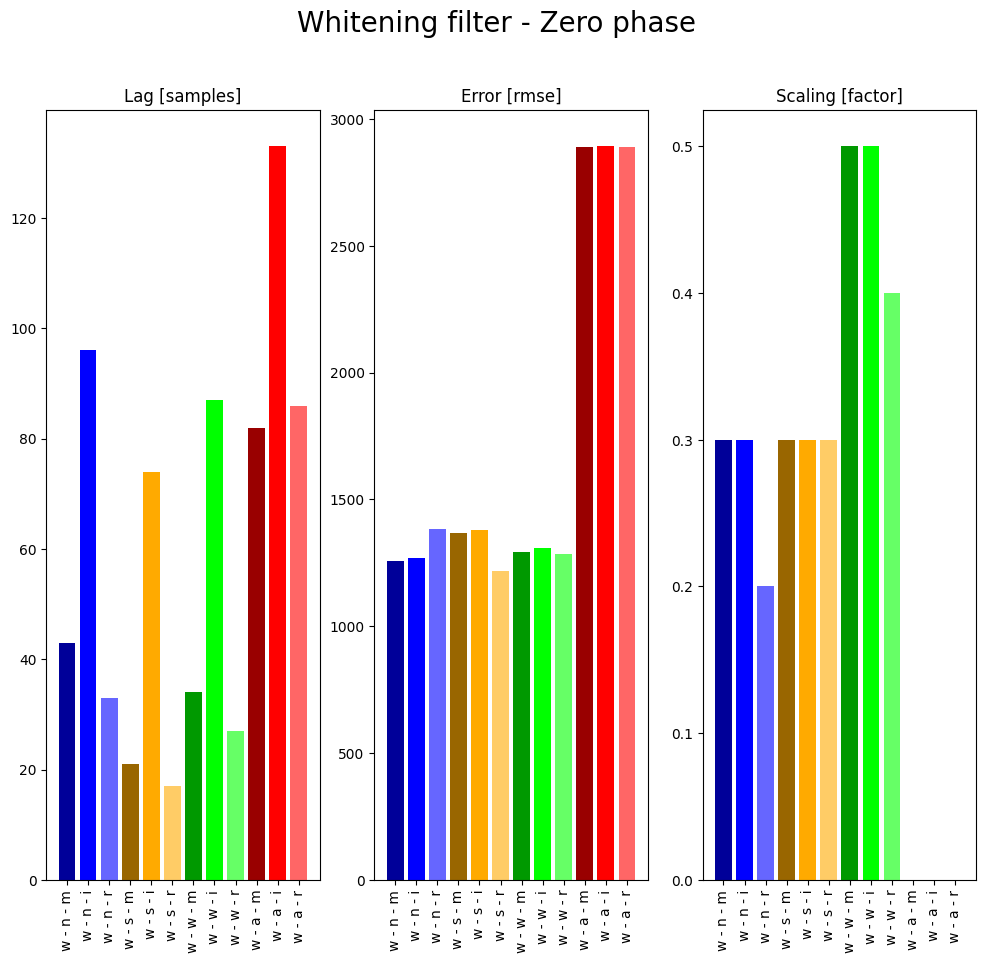
\includegraphics[width=1.0\columnwidth]{images/result_whitening_zerophase.png}
	\end{center}
	\caption{Lag, error, and scaling of different filtering and envelope techniques with whitening applied. The whitening filter is constructed from the desired frequency amplitude response and a phase. The frequency response is determined as described in the simulation section \ref{sec:whitening}, and the phase is set to zero phase. The abbreviations are the first letter of the used technique for each step. Further clarification of these abbreviations can be found in Table~\ref{tab:abbreviation_explanation}}
	\label{fig:result_whitening_zerophase}
\end{figure}